% !TEX encoding = UTF-8
% !TEX program = xelatex
\documentclass[12pt,a4paper]{article}
\usepackage[paperwidth=210mm, paperheight=297mm, left=0.75in, right=0.75in, bottom=1in, top=1in]{geometry}
\usepackage{polyglossia}
\setdefaultlanguage[babelshorthands]{italian}
\usepackage{fontspec}
\usepackage{graphicx}
\usepackage{blindtext}
\usepackage{wrapfig}

\frenchspacing
\makeindex

\begin{document}
\title{\vspace{-70pt}Wilkinson Microwave Anisotropy Probe (WMAP)}
\author{Davide Piona}
\date{}
\maketitle
\pagestyle{empty}
\thispagestyle{empty}

\section*{Storia}
\label{storia}
\begin{wrapfigure}{r}{0.35\textwidth}
  \vspace{-10pt}
  \begin{center}
    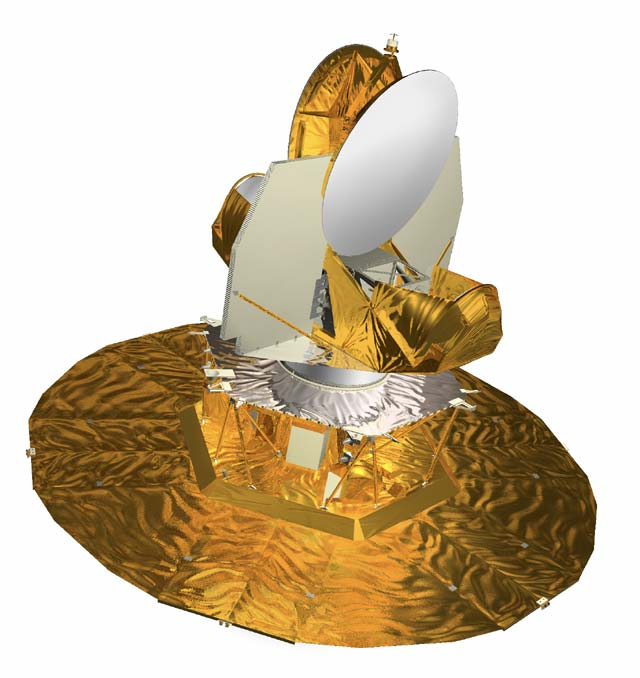
\includegraphics[width=0.30\textwidth]{satellite}
  \end{center}
  \vspace{-20pt}
\end{wrapfigure}

Data di lancio: 30 giugno 2001\\
Sito di lancio: Cape Canaveral, Stati Uniti\\
Destinazione: Punto di Lagrange L2\\

La missione MAP venne proposta alla NASA nel 1995 con lo scopo di misurare le differenze di temperatura nella \emph{radiazione cosmica di fondo}. Il WMAP è stato preceduto da altri due satelliti: il RELIKT--1 e il COBE. 

Originariamente il WMAP avrebbe dovuto completare le prime osservazioni dopo due anni ma estensioni della missione sono state garantite nel 2002, nel 2004 e nel 2009, dando così alla sonda una vita totale di 9 anni; tale missione è terminata nel mese di settembre del 2010. Ad ottobre del 2010, la sonda è stata portata verso l'orbita cimitero, concludendo così il suo compito.

La successiva sonda spaziale sviluppata a tale scopo è il Planck Surveyor, il cui lancio è avvenuto il 14 maggio 2009.

\section{Osservazioni}
\label{osservazioni}

Gli specchi primari del WMAP sono grandi 1,4 metri e 1,6 metri e sono rivolti in direzioni opposte tra loro; questi focalizzano il segnale ottico su specchi secondari grandi 0,9 m x 1,0 . La base del WMAP è costituita da un pannello solare di 5 metri di diametro.

Il WMAP raccoglie dati in cinque lunghezze d'onda differenti, permettendo così di eliminare varie radiazioni contaminanti la radiazione di fondo.

Il WMAP ha fornito un'immagine dettagliata dell'universo e ha scoperto che l'universo ha un'età di 13,75 miliardi di anni; inoltre è composto di:

\begin{itemize}
\item \textbf{energia oscura} per il 71,2\% (con un errore del 1,5\%)

\item \textbf{materia oscura} per il 23,3\% (con un errore del 1,3\%)

\item \textbf{materia} per il 4,4\% (con un errore del 0,9\%)

\end{itemize}

\section{Curiosità}
\label{curiosit}

Il WMAP, rispetto al suo predecessore COBE, ha una sensibilità 45 volte superiore, ed una risoluzione angolare 33 volte più precisa.

Il posizionamento dell'orbita del WMAP al punto di Lagrange 2 (1,5 milioni di km circa dalla Terra), minimizza le emissioni di interferenza provenienti dal Sole, dalla Terra e dalla Luna, permettendo anche una stabilità termica degli strumenti.

\end{document}